

\section{METHODOLOGY}

\subsection{Data Collection}
For a project data is the most important part that may be of various forms such as text, audio, video etc. In our case we required the audio data
as it deals with the recognition of voice from the user to interact with 
system.Thus large samples of data are required for the training of the 
model and hence enhance the performance ability of the recognition model.
The Data collection phase is the initial phase of the project to 
begin with. This stage has been divided to two phases as discussed below:

\subsubsection{Sample Voice Collection}
In collecting required data for the project we needed the Nepali spoken 
words as we were dealing for the interactive voice response system
using Nepali speech. The sources for Nepali speech data were not available
in the web so that we had to manually collect the data from the individuals
The sample voice collection was done from several individual possible.
\begin{figure}[h]
	\begin{center}
		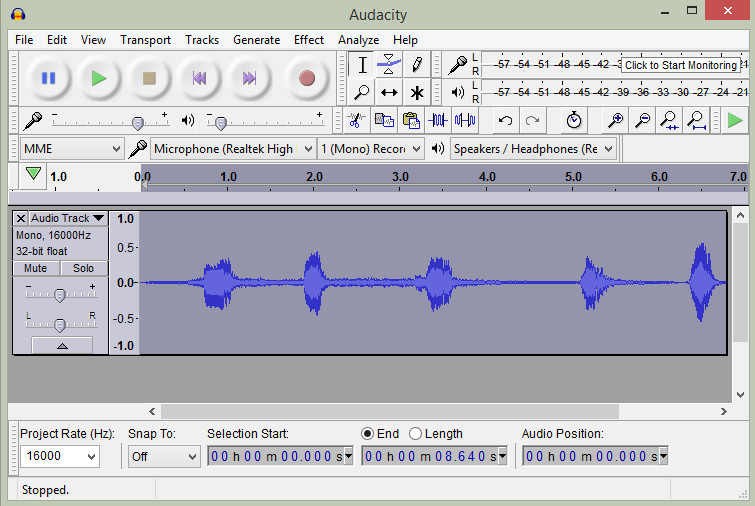
\includegraphics[scale=0.7]{images/audacity.png}
		\caption{Audacity Interface for sound sample recording}
		\label{audacity}
	\end{center}
\end{figure}


For recording purpose we used a simple software called "Audacity", which
is free and cross platform software Licensed under the GNU General Public License (GPL).
It easily runs on several platforms such as Windows, Mac OS X/mac OS and GNU/Linux.
Audacity can record live audio through a microphone or mixer, 
or digitize recordings from other media. With some sound cards, and on 
any recent version of Windows, Audacity can also capture streaming audio. 
Thus for collecting sound samples we developed a simple tutorial on
recording the speech and collected data from several individuals and also manually 
recorded the voices.As our Devanagari script is very vast for the preliminary stage 
we are working with the simple sound samples from numbers 0 to 9. For our
project we used the sound samples of  frequency rate of 16000Hz recorded using
the mono-channel configuration.Similarly we used 16-bit samples for the project.
The sample voice collected thus were used for the training data generation.



\subsubsection{Training Data Generation}
After collecting the sample voices from multiple sources, we need to create training samples to be used in speech recognition. The sample voice contains speech signals numbered from $0 - 9$. Now these samples need to be separated into individual files each containing a digit so that it can be used as training samples. 

To generate sample of each digit, we have to detect silence zones from the sample file and separate each based on those silence regions.

Now, to detect the silence zones, it \textquotesingle  s highly depended on the audio signal. We need to detect the threshold level, below which the sound can be considered as silent. In order to detect the threshold level, first we fragment the whole audio sample into certain number of frames based on sample width. Then, we calculate the root mean square value which gives an approximate estimate of threshold level, below which the sound frames can be considered silence and above it as voiced activity.

After the detection of threshold level, we need to partition the sound sample. Based on the threshold level for a sound sample, now we detect the silent zones, and thereafter the ranges. We define a minimum silence length in second. And the audio sample is fragmented into number of sample per frame based on silence length. If a frame \textquotesingle s rms value is less than threshold then, the frame is considered as silent frame, and so on silent ranges are determined. These ranges can be complimented then to generate the ranges that actually contains the voice. Then the audio sample is partitioned based on these non-silence activity ranges.
\begin{figure}[h]
	\begin{center}
		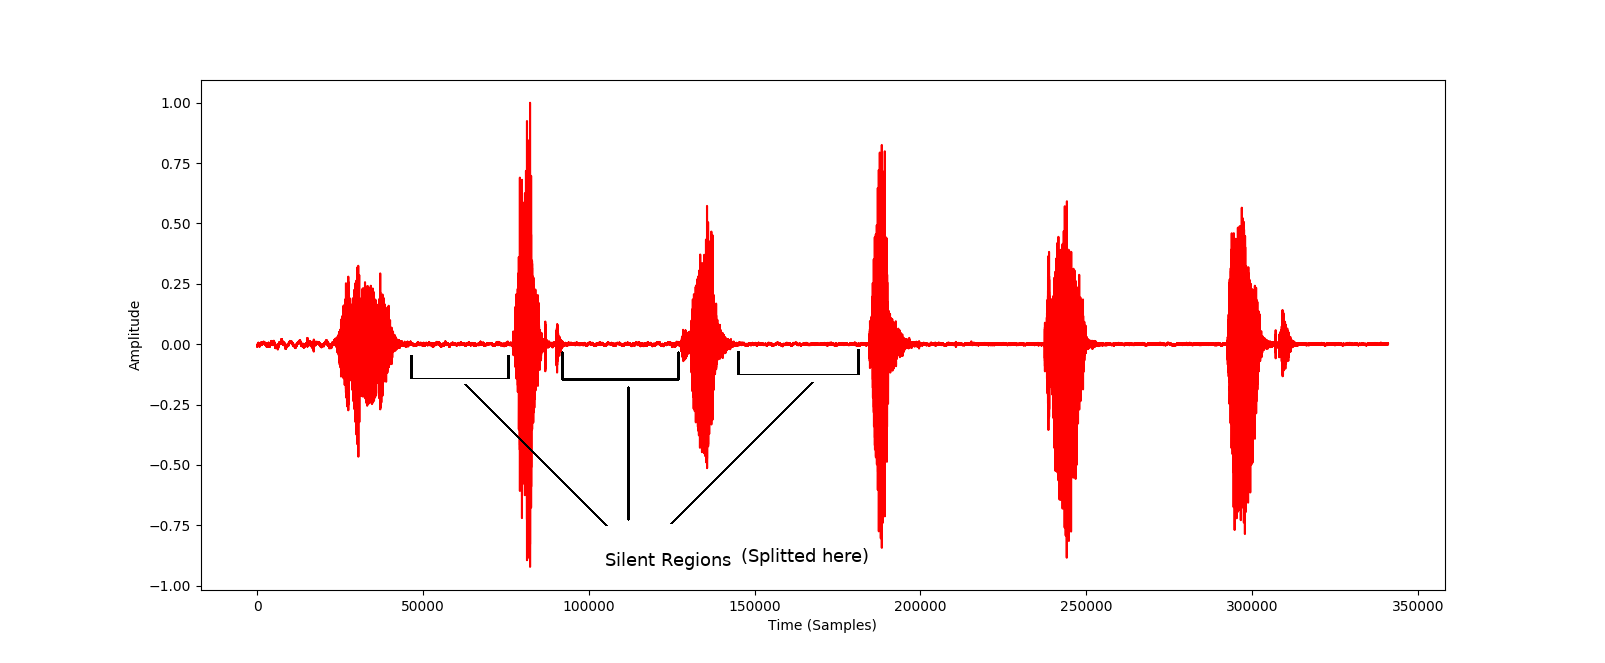
\includegraphics[width=6in]{images/sample.png}
		\caption{Training samples generation from recorded voice}
		\label{sample}
	\end{center}
\end{figure}

\subsection{Noise Reduction}

The speech signal may contain some noise. Actually, most of the speech signals contains background noise. This noise degrades the quality of the speech signal and create hindrance in the processing the speech. Thus, a noise reduction algorithm is needed to reduce the noise level without affecting the speech signal quality. One of the noise reduction algorithm used in this project is Spectral Subtraction method. It is performed independently in the frequency bands corresponding to the auditory critical bands.

The spectral subtraction method is a simple and effective method of noise reduction. In this method, an average signal spectrum and average noise spectrum are estimated in parts of the recording and subtracted from each other, so that average signal-to-noise ratio (SNR) is improved. It is assumed that the signal is distorted by a wide-band, stationary, additive noise, the noise estimate is the same during the analysis and the restoration and the phase is the same in the original and restored signal.

The noisy signal y(m) is a sum of the desired signal x(m) and the noise n(m):
\begin{equation}
y(m) = x(m) + n(m)
\end{equation}

In the frequency domain, this may be denoted as:
\begin{equation}
Y(j\omega) = X(j\omega) + N(j\omega) \Rightarrow X(j\omega) = Y(j\omega) – N(j\omega)\\
\end{equation}
where $Y(j\omega), X(j\omega), N(j\omega)$ are Fourier transforms of y(m), x(m), n(m), respectively.
To take the Discrete Fourier Transform of the frame, perform the following:
\begin{equation}
Y_i(k) =
\sum_{m=1}^{N}
y_i(m)h(m)e^{-j2\pi km/N} \qquad 1\leq k\leq K\\
\end{equation}

where $h(m)$ is an N sample long analysis window (e.g. hamming window), and K is the length of the DFT. The magnitude spectrum for the speech frame $y_i(m)$ is given by:

\begin{equation}
M_{i}(k) = | Y_{i}(k) |
\end{equation}

The phase spectrum is calculated in the following way:
\begin{equation}
\theta_i(k) = tan^{-1}(\frac{Im(Y_i(k))}{Re(Y_i(k))}) \\
\end{equation}


The statistic parameters of the noise are not known, thus the noise and the speech signal are replaced by their estimates:

\begin{equation}
\hat{X}(j\omega) = Y(j\omega) - \hat{N}(j\omega)\\
\end{equation}

Noise is the time-average estimate of first few frames of the speech signal.
\begin{equation}
\hat{N}(j\omega) = \frac{1}{K}  \sum_{i=0}^{K-1}|N_i(j\omega)| \\
\end{equation}

The noise reduced clean speech signal is then obtained by performing the inverse Fourier transform of $X(j\omega)$
\begin{figure}[h]
	\begin{center}
		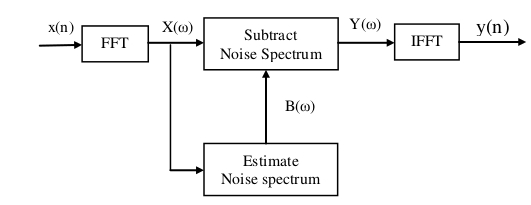
\includegraphics[width=6in]{images/noise.png}
		\caption{Noise removal process in speech signal}
		\label{noise}
	\end{center}
\end{figure}


The procedural Explanation of the noise removal technique of the input speech signal is discussed below:

The basic principle is as follows: if we assume additive noise, then we can subtract the noise spectrum from the noisy speech spectrum, so we are left with what should look like the clean speech spectrum. For this we need to know what the noise spectrum looks like, so we estimate it during regions of no speech (parts of the signal that contain only noise) and then assume it won't change much from frame to frame.

Let's assume a clean time domain signal, $x(m)$ to which we add additive noise, $n(m)$.The signal we actually see is the sum $y(m) = x(m) + n(m)$. We wish to estimate the true value of $x(m)$ given $y(m)$ only.

The first step in spectral subtraction is to frame the speech signal into short, overlapping frames. Typically frames are taken to be about 20ms long. For a 16KHz sampled audio file, this corresponds to $$0.020s * 16,000 samples/s = 320\enspace samples$$ We then use an overlap of 50\%, or about 200 samples. This means the first frame starts at sample 0, the second starts at sample 200, the third at 400 etc.

Then, we need a window, which contains certain number of frames. We used Hamming window for this project. We then take the discrete Fourier transform of each frame and extract the magnitude and phase spectrum from each. Let $y_i(m)$ be framed time domain signal and $Y_i(k)$ is its complex Discrete Fourier Transform, (DFT) where m ranges over 1-400 (if our frames are 400 samples ) and $i$,  ranges over the number of frames. Then $M_i(k)$ is the magnitude spectrum of frame $i$.

We used Fast Fourier Transform (FFT) in real world practice.
The magnitude spectrum for the speech frame $y_i(m)$ is given by:
\begin{equation}
M_i(k) = |(Y_i(k)|
\end{equation}


\vspace{9mm}
\begin{lstlisting}
Pseudocode
windowed_frame = frame .* hamming(length(frame));
complex_spec = fft(windowed_frame,512); 
mag_spec = abs(complex_spec);
phase_spec = angle(complex_spec);
\end{lstlisting}


Now, to get the estimate of noise, a common assumption is that the first few frames of an audio signal consist of silence.To get our noise estimate, we can take the mean of the first few or so frames. With the magnitude and noise estimate for each frame, now we proceed with spectral subtraction: subtraction of noise estimate. It can be done as:
\begin{equation}
\hat{M}_i(k) =
\begin{cases}
	M_i(k) - N_i(k)\qquad if\enspace M_i(k) \geq N_i(k)\\
	0 \hspace{3cm} if\enspace M_i(k) < N_i(k)\\
\end{cases}
\end{equation}


Here, $\hat{M}_i(k)$ is the estimated clean spectrum. $M_i(k)$ is the noisy spectrum. And $N_i(k)$ is the noise estimate.

Note that we restrict our estimated magnitude spectrum to be positive, since magnitude spectrum must be.

\begin{lstlisting}
clean_spec = mag_spec - noise_est;
clean_spec(clean_spec < 0) = 0;
\end{lstlisting}

Now we have an estimate of the clean spectrum for every frame. With this, we would like to reconstruct the original audio recording which will  have less background noise. For this we use the clean spectrum $M_i(k)$ and phase spectrum from each frame that we calculated at the beginning.

Then, the estimated clean complex spectrum for each frame $Y_i(k)$ (enh\_spec) is


\begin{lstlisting}
enh_spec = clean_spec.*exp(j*phase_spec)

\end{lstlisting}



Now, Inverse FFT (IFFT) of $\hat{Y}_i(k)$ is calculated to reconstruct our original signal $\hat{x}(m)$ and do overlap add of the resulting time-domain frames.



\subsection{Feature Extraction}
The goal of feature extraction is to transform the input waveform into a sequence of \textbf{feature vectors}, each vector representing the information in a small time window of the signal. The most commonly used feature extraction is the \textbf{MFCC, the Mel Frequency Cepstral Coefficients}. These are based on the important idea of cepstrum. The steps in MFCC are shown in Fig 3.4 and described in following sections. 

\begin{figure}[h]
	\begin{center}
		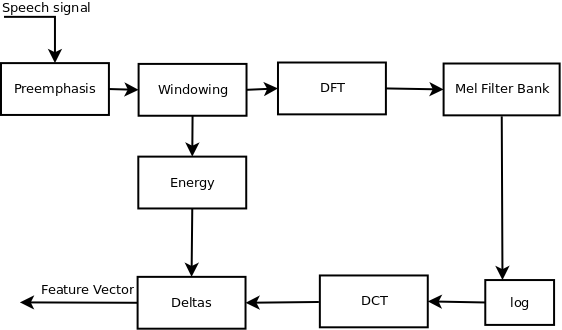
\includegraphics[scale=0.3]{images/feature-blockdiagram.png}
		\caption{Stages in feature extraction}
		\label{feature}
	\end{center}
\end{figure}

\subsubsection{Preemphasis}
The first stage in MFCC feature extraction is to boost the amount of energy in the high frequencies. The spectrum of voiced segments for vowels shows that there is more energy at the lower frequencies than the higher frequencies. This drop in energy across frequencies is called spectral tilt and is caused by the nature of the glottal pulse. Boosting the high frequency energy makes information from these higher formants more available to the acoustic model.
\begin{figure}[h]
	\centerline{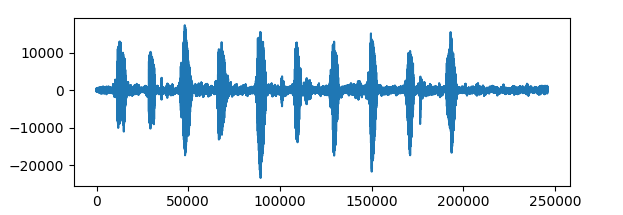
\includegraphics[scale=0.50]{images/beforepreemphasis.png}}
	\caption{Speech signal before pre-emphasis}
\end{figure}

\begin{figure}[h]
	\centerline{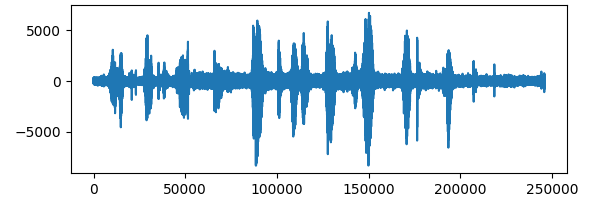
\includegraphics[scale=0.50]{images/afterpreemphasis.png}}
	\caption{Speech signal after pre-emphasis}
\end{figure}

\subsubsection{Windowing}
Speech signal are non-stationary signals, meaning that their statistical properties are not constant across time. So, we take spectral features from a small window of speech signal so that we can make an assumption that the signal is stationary (i.e. the statistical properties are constant within the region).The extraction of the signal takes place by multiplying the value of the signal at the time n, \textit{s[n]}, with the value of the window at time n, \textit{w[n]}:
\begin{equation}
y[n] = w[n]s[n]
\end{equation}

We can characterize the windowing process by three parameters : how \textbf{wide} is the window, what is the \textbf{offset} between the successive windows and what is the \textbf{shape} of the window.
We call the speech extracted  from each window a \textbf{frame}, the number of milliseconds in the frame the \textbf{frame size} and the number of milliseconds between the left edges of the successive windows the \textbf{frames shift step}.

The signals are framed into 20-40ms. We have used frames of frame size 25ms. So, for a signal with 16 KHz signal, we have 0.025*16000 = 400 samples. The frame step is taken as 10ms i.e. 160 samples. This allows for overlapping of the frames. The first 400 samples start at sample 0, the next starting at sample 160, etc. until end of the signal is reached.

\subsubsection{Discrete Fourier Transform}
The next step to extract information from the frames; we need to know how much energy the signal contains at different frequency bands. For this, we use Discrete Fourier Transform (DFT).

The input to the DFT is a windowed signal \textit{x[n]...x[m]}. To take the DFT of the frame, we perform the following:
\begin{equation}
S_i(k) = \sum_{n=1}^{N}s_i(n)h(n)e^{\frac{-j2 \pi kn}{N}}\quad\quad  1\leq k\leq K 
\end{equation}


where h(n) is an N sample long analysis window and K is the length of the DFT.


The peridiogram-based power spectral estimate for the frame $s_i$(n) is given by
\begin{equation}
P_i(k) = \frac{1}{N}|S_i(k)^2 
\end{equation}

\subsubsection{Mel Filter Bank}
The results of FFT will be amount of energy at each frequency band. Human hearing, however, is not equally sensitive at all frequency bands. It is less sensitive at higher frequencies, roughly above 1000 Hz. The modelling of this human hearing property during feature extraction improves speech recognition performance. The form of the model used in MFCCs is to warp the frequencies output of the FFT onto the mel scale. A \textbf{mel} is a unit of pitch defined so that the pairs of sounds perceptually equidistant in pitch are separated by an equal number of mels. The mapping between frequency in Hz and the mel scale is linear below 1000 Hz and logarithmic above 1000 Hz. The mel frequency m can be computed from frequency as 
\begin{equation}
mel(f)=1127ln(1+\frac{f}{700})
\end{equation}
The filter bank is a set of 20-40 (26 is standard) triangular filters applied to the periodogram power spectral estimate. For 26 filters, we get 26 vectors. The Mel-spaced filterbanks can be computed from the following equations


\begin{equation}
	H_m(k) =
	\begin{cases}
		0 & k<f(m-1) \\
		\frac{k - f(m-1)}{f(m) - f(m-1)} & f(m-1) \leq k \leq f(m) \\
		1 & k = f(m)\\
		\frac{f(m+1) - k }{f(m+1) - f(m)} & f(m) \leq k \leq f(m+1) \\
		0 & k>f(m+1)
	\end{cases}
\end{equation}

where M is the number of filter we want.    
To calculate the filterbank energies, each filterbank is multiplies with the power spectrum, then added up. This provides the energy in each filterbanks.


Finally, we take the log of each of the mel spectrum values. In general, the human response to the signal level is logarithmic; human are less sensitive to slight differences in amplitude at high amplitudes than at low amplitudes. In addition, using a log makes the feature estimates less sensitive to variations in input.
\begin{figure}[h]
	\centerline{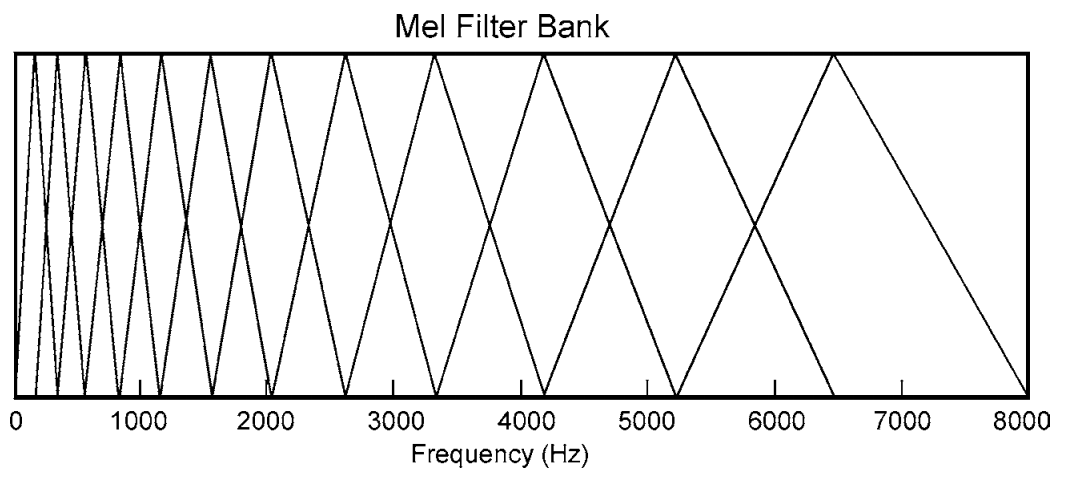
\includegraphics[scale=0.35]{images/filterbanks.png}}
	\caption{Mel filter Bank}
\end{figure}


\subsubsection{Discrete Cosine Transform}
The final step is to compute Discrete Cosine Transform (DCT) of the log filterbank energies. The filterbank energies are quite correlated with each other as our filterbanks are overlapping. The DCT decorrelates the filter bank coefficients and yield a compressed representation of the filter banks.

\subsubsection{Deltas and Energy}
The extraction of the cepstrum via DCT results in cepstral coefficients for each frame. The energy within a frame is also an important feature that can added to the cepstral coefficients. We usually add the the log energy to the cepstral coefficients.


We also can add a delta or velocity feature to the cepstral coefficients for better performance. The delta features represents the change between frames in the corresponding cepstral/energy features. The deltas can be computed from the difference between frames; thus the delta value \textit{d(t)} for a particular cepstral value \textit{c(t)} for time \textit{t} can be estimated as
\begin{equation}
d(t) = \frac{\sum_{n=1}^{N}n(c(t+n) - c(t-n))}{2 \sum_{n=1}^{N}n^2}
\end{equation}


\subsection{Prediction}

Prediction refers to predicting the sound samples based on the Features Extracted. Prediction is done first by teaching a model from the data sets that we have and then making it to predict for new inputs. The Speech Recognition for IVR system is an Isolated Word Recognizer problem. The MFCC features obtained from above for each time frames act as the data sources that can be feed to train the model and later on predict from the model. Prediction is done by using Hidden Markov Models and Recurrent Neural Networks. These both are different approaches but with both approaches implied we can compare both and select the best one.


\subsubsection{Hidden Markov Model}


A hidden Markov model is defined as a pair of stochastic processes ($X$,$Y$). The $X$ process is
a first order Markov chain, and is not directly observable, while the $Y$ process is a sequence
of random variables taking values in the space of acoustic parameters, or observations.

Let $y$ $\epsilon$  $Y$ be a variable representing observations and $i$ , $j$ $\epsilon$  $X$ be a variable representing model states, the model can be represented by following parameters

\[ A = \{a _{i,j} | i,j \epsilon X \} \hspace{1cm}   Transition Probabilities \]
\[ B = \{b _{i,j} | i,j \epsilon X \} \hspace{1cm}   Output Distributions \]
\[  \Pi  = \{\pi _{i} | i \epsilon X \}  \hspace{1cm}  Initial Probabilites \]


with the following definitions:

\begin{equation} a _{i,j} = P(X _{t} = j | X _{t-1} = i ) \end{equation}
\begin{equation} b _{i,j}(y) = P(Y _{t} = y | X _{t-1} = i ,  X _{t} = j ) \end{equation}
\begin{equation} \pi _{i} = p(X _{0} = i) \end{equation}

For convenience, the HMM is generally represented in a complex notation
\begin{equation} \lambda = (A,B, \Pi ) \end{equation}

\paragraph{Evaluation} \mbox{}\\
Evaluation in HMM refers to efficiently computing $ P(O|\lambda) $, the probability of the observation sequence, given the observation sequence $ O = (0 _{1}, 0 _{2},0 _{3},...,0 _{n}) $ and an HMM model $ \lambda = (A,B, \Pi ) $. This can be solved by using either of the procedure from the Forward-Backward Procedure.
\subparagraph{The Forward Procedure:}
One way to calculate $ P(O|\lambda) $ given $ \lambda $ is to enumerate all possible combinations. Considering that there are N total observable symbols at each state and we
wish to calculate the probability of observation sequence $ O = (o _{1}, o _{2},o _{3},...,o _{n}) $, There will be $ N^{T} $ state sequences. And, calculating the probability for each such sequence would require $(2T -1)$ multiplications and in total we would require $(2T -1) * N^{T} $ multiplications and $ N^{T} $ additions.This is inefficient and a more efficient algorithm is required. Forward algorithm is
an efficient algorithm for this. Consider the forward variable: 

\begin{equation} \alpha _{t} (i) = P(o _{1}, o _{2},o _{3},...,o _{t},q(t) = i|\lambda)  \end{equation}

that is the probability of the partial observation sequence, $o _{1}, o _{2},o _{3},...,o _{t}$ (until time t) and
state $i$ at time $t$, given the model $\lambda$. We can solve for $\alpha _{t} (i)$ inductively as follow.
\begin{enumerate}
	\item Initialization 
	\begin{equation} \alpha_{1}(i) = \Pi_{i}b_{i}(o_{i}), 1 \leq i \leq N  \end{equation}
	
	\item Induction
	\begin{equation} \alpha_{t+1}(j) = \{ \sum_{i=1}^{N}\alpha_{t}(i)a(i,j) \} b_{j}(i)(o_{t+1}) ,1 \leq t \leq T-1 ; 1 \leq j \leq N \end{equation}
	
	\item Termination
	\begin{equation} P(O|\lambda) = \sum_{i=1}^{N} \alpha_{T}(i) \end{equation}
\end{enumerate}

\subparagraph{The Backward Procedure:}
In a similar manner, we can consider a backward variable $ \beta_{t}(i) $ defined as 

\begin{equation} \beta _{t} (i) = P(o _{t+1}, o _{t+2},o _{t+3},...,o _{T},q(t) = i|\lambda)  \end{equation}

that is the probability of the partial observation of sequence from t+1 to end, given state $i$ at time $t$ and the model $\lambda$. We can solve for $\beta _{t} (i)$ inductively as follow.
\begin{enumerate}
	\item Initialization 
	\begin{equation} \beta_{T}(i) = 1, 1 \leq i \leq N  \end{equation}
	
	\item Induction
	\begin{equation} \beta_{t}(i) =  \sum_{j=1}^{N}a(ij) b_{j}(o_{t+1})\beta_{t+1}(j) , t = T-1, T-2, ... , 1  and  1 \leq i \leq N \end{equation}
	
\end{enumerate}

\paragraph{Decoding} \mbox{}\\
Decoding refers to finding or choosing  a state sequence $ Q = (q_{1},q_{2},q_{3},...,q_{n}) $ that best explains the observation sequence $ O = (o_{1},o_{2},o_{3},...,o_{n}) $ for an HMM model $ \lambda = (A,B, \Pi ) $. This problem can be solved by using the Forward-Backward algorithm too but the Viterbi algorithm is the most widely used solution to this "Optimal State" problem. To find the state sequence $ Q = (q_{1},q_{2},q_{3},...,q_{n}) $ for the observation sequence $ O = (o_{1},o_{2},o_{3},...,o_{n}) $ , We need to define the quantity :
\begin{equation} \delta_{t}(i) = max(q_{1},q_{2},q_{3},...,q_{t-1})P(q_{1},q_{2},q_{3},...,q_{t-1},q_{t}=o_{1},o_{2},o_{3},...,o_{t}) | \lambda \end{equation}
This is, $\lambda_{t}(i)$ is the best source along a single path, at time t, which
accounts for the first $t$ observations and ends in state $i$. By induction, we have
\begin{equation} \delta_{t+1}(j) = max(i)[\delta_{t+1}(j)a(ij)]b_{j}(o_{t+1}) \end{equation}

To actually retrieve the state sequence we need to keep track of the arguments that
maximized the above equation, for each $t$ and $j$. We do this via the array $\Psi_{t}(j)$.The complete
procedure for finding the best state sequence can now be stated as follow.

\begin{enumerate}
	\item Initialization
	\begin{equation} \delta_{t}(i) = \Pi_{i}b_{i}(o_{t}) , 1 \leq i \leq N \end{equation}
	\begin{equation} \Psi_{1}(j) = 0 \end{equation}
	
	\item Recursion
	\begin{equation} \delta_{t}(i) = max(1 \leq i \leq N)[\delta_{t-1}(i)a(ij)]b_{j}(o_{t}), 1 \leq j \leq N , 1 \leq t \leq T \end{equation}
	\begin{equation} \Psi_{t}(j) = argmax(1 \leq i \leq N)\delta_{t-1}(i)a(ij), 1 \leq j \leq N , 1 \leq t \leq T \end{equation}
	
	\item Termination
	\begin{equation} P = max(1 \leq i \leq N) [\delta_{T}(i)] \end{equation}
	\begin{equation} q_{T} = argmax(1 \leq i \leq N) [\delta_{T}(i)] \end{equation}
	
	\item Backtracking
	\begin{equation} q_{t} = \Psi_{t+1}(q_{t+1}), t = T-1, T-2,...,1 \end{equation}
\end{enumerate}
The above algorithms are implemented in log scale because of low values of probability.
Also, it is worth noting that viterbi algorithm is similar to forward implementation of the
forward procedure except some subtle differences.

\paragraph{Learning} \mbox{}\\

Learning refers to adjusting the model parameters $ \lambda = (A,B, \Pi ) $ to maximize $ P(O|\delta)$. This is the most difficult problem of HMMs. The algorithm used for this step is the buam-welch algorithm. Baum-Welch re-estimation uses EM (Expected maximization) to determine the HMM parameters.

\begin{enumerate}
	\item Define $\xi(i,j)$ as probability of being in state $i$ at time $t$, and in state $j$ at time $t+1$
	
	\[ \xi(i,j) = \frac{\alpha_{t}(i)a_{ij}b_{j}(O_{t+1})\beta_{t+1}(j)}{P(O|\lambda)} \]
	
	\begin{equation} = \frac{\alpha_{t}(i)a_{ij}b_{j}(O_{t+1})\beta_{t+1}(j)}{\sum_{i=1}^{N} \sum_{j=1}^{N} \alpha_{t}(i)a_{ij}b_{j}(O_{t+1})\beta_{t+1}(j)}  \end{equation}
	
	\item Define $\gamma_{t}(i)$ as the probability off being in state $i$ at time $t$, given the observation sequence.
	
	\begin{equation}
	\gamma_{t}(i) = \sum_{j=1}^{N} \xi(i,j) \end{equation}
	
	\item So, $\sum_{t=1}^{T} \gamma_{t}(i)$ is the expected number of times state $i$ is visited, and $\sum_{t=1}^{T-1}\xi_{t}(i,j)$ is the expected number of transitions from state i to state j.
	
	\item Now the parameters of HMM are updated as \\
	$\Pi_{i} = $ Expected frequency in state $i$ at time $t = 1 = \gamma_{1}(i)$\\
	$a_{ij} = $ (expected number of transition from state i to state j) / (expected number of transition from state i) :
	
	\begin{equation} a_{ij} = \frac{\sum \xi_{t}(i,j)}{\sum \gamma_{t}(i)} \end{equation}
	$b_{j}(k) = $ (expected number of times in state j and observing symbol k) / (expected number of times in state j):
	
	\begin{equation} b_{j}(k) = \frac{\sum_{t,ot=k} \gamma_{t}(j)}{\sum_{t}\xi(j)} \end{equation}
\end{enumerate}

Continuous observation densities in HMMs When introducing HMM, we defined the observations of the HMMs to be discrete symbols from a finite alphabet, and therefore we could use a discrete probability density within each state of this model. These are called discrete HMMs. The problem with this approach is that the observations are often continuous in most of the practical applications. Although it is possible to convert such continuous signal representations into a sequence of discrete symbols via vector quantization codebooks etc, there might be serious degradation associated with such discretization of the continuous signal. Hence, it would be advantageous to be able to use HMMs with continuous observation densities to model continuous signal representations directly.

To use continuous observation density, some restrictions must be placed on the form of the model probability density function (pdf) to ensure that the parameters of the pdf can be re-estimated in a consistent way. The most general representation of the pdf, for which a re-estimation procedure has been formulated, is a finite mixture of the form
\begin{equation} b_{j}(o) = \sum_{k=1}^{M}C(jk)N[O,\mu_{jk},U_{jk}] , 1 \leq j \leq N \end{equation}

Where $O$ is the observation vector being modeled. $c_{jk}$ is the mixture coefficient for the $kj^{th}$ mixture in the state $j$ and $N$ is any log-concave or elliptically symmetric density. The mostly used distribution is the Gaussian distribution. The equations of a multivariate gaussian distribution for independent random variables is where $\mu_{j}$ is the mean vector, and
the covariance matrix $U_{jk}$ reduces to $\sigma_{ii}$ , the product

\begin{equation} f(X=x|\mu,\textstyle \sum) = \prod_{i=1}^{N} \frac{1}{(2\pi)^{\frac{1}{2}}} exp {- \frac{(x_{i}-\mu_{i})^{2}}{2\sigma_{ii}^{2}}}  \end{equation}

of the covariance matrix.

\subsubsection{Recurrent Neural Network}

A recurrent neural network (RNN) is a class of artificial neural network where connections between units form a directed cycle. Due to this Recurrent Neural Network can be used for temporal data classification like speech classification. RNN has been implemented and to remove the vanishing gradient problem both the LSTM and GRU variants of RNN has been implemented.





\begin{figure}[h]
	\begin{center}
		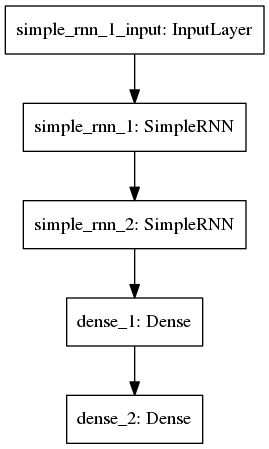
\includegraphics[scale=0.6]{model_simple}
		\caption{RNN implementation}
		\label{audacity}
	\end{center}
\end{figure}



